\subsection{Production}

Im Gegensatz zu einem Research Honeypot wird ein Production Honeypot, wie der Name schon sagt, in einem produktiven Umfeld eingesetzt. Eine mögliche Implementierung ist in Abb. \ref{hnet:prodhon} zu sehen. Ziel eines Production Honeypots ist es, das Netzwerk sicherer zu machen. Er soll dafür sorgen die Infrastruktur vor Angriffen zu schützen und die Aufmerksamkeit der Angreifer auf sich zu lenken. 
\\
\begin{figure}[ht]
    \centering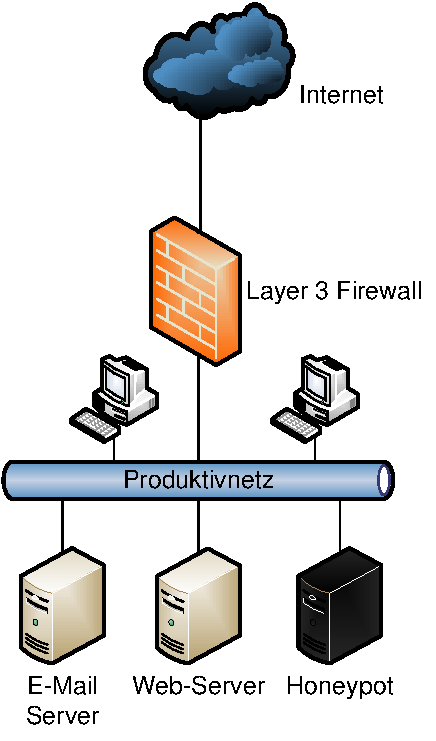
\includegraphics[scale=0.6]{Bilder/produktiv.pdf}
  \caption{Production Honeypot}
  \label{hnet:prodhon}
\end{figure}
\\
Um die Wirkung des Honeypots genauer zu beschreiben, werden im folgenden die drei Kategorien von \glqq Sicherheit\grqq, welche von ---Verweiß--- definiert wurden, aus Sicht des Honeypots erläutert. 

\\
\begin{itemize}							% Beginn der Aufzählungsumgebung
\item{\textbf{Verhütung (Prevention)}} 

Um ein Netzwerk vor einem Angriff zu schützen werden häufig Firewalls und andere Sicherheits-Systeme eingesetzt. Ein Honeypot wird jedoch selten eingesetzt um sich vorbeugend vor Angriffen zu schützen. Sobald ein Honeypot aktiv wird, ist der Angreifer bereits in das Netzwerk bzw. System eingedrungen. Wenn der Honeypot falsch konfiguriert ist, wird er sogar zu einer Gefahr für das eigene Netzwerk und zu einer Eingangstür für Angreifer. Trotz alle dem gibt es auch Punkte, die für einen Honeypot als vorbeugende Sicherheitsmaßnahme sprechen.

Zum einen werden die Angreifer verunsichert, da sie über die Existenz der Honeypots wissen. Bricht ein Angreifer in ein System ein, muss er sicher immer bewusst sein, dass er möglicherweise gerade in eine Falle gelockt wurde. Diese Tatsache könnte Angreifer verunsichern und von größeren Netzwerken fernhalten. 

Des Weiteren kann argumentiert werden, dass ein Angriff auf einen Honeypot den Schaden von produktiven Systemen vorbeugend abwehrt. Der Honeypot beschäftigt den Angreifer und führt ihn meist für eine längere Zeit in die Irre. In dieser Zeit kann der Angreifer an keine wichtigen Daten gelangen und der eigentliche Angriff auf die produktiven Systeme wird dadurch verhindert. Dieser Aspekt zur Sicherung produktiver Daten kann ebenfalls als ein vorbeugender Schutz gesehen werden.   
\item{\textbf{Erkennung (Detection)}}

Im Gegensatz zu der Angriffs-Verhütung ist der Honeypot für die Erkennung von Angriffen besser geeignet. In einer Demilitarisierten Zone (DMZ) eines Netzwerks sind Systeme, welche meist mit dem Internet verbunden sind. Durch diese Verbindung ist das Risiko eines Angriffs an dieser Stelle erhöht. Wird hier ein Honeypot, wie es in Abb. \ref{hnet:prodhon} gezeigt, implementiert, kann dieser als eine Art Alarmanlage dienen. Da ein Honeypot nicht aktiv im Netzwerk arbeitet und somit auch keine Systeme eine Verbindung mit dem Honeypot benötigen, sollte es keine Verbindungsversuche geben.
Bei Verbindungsversuchen auf Ports welche typischerweise für Internetdienste verwendet wird, handelt es sich meist um einen Port-Scan eines potenziellen Angreifers. Dieser versucht damit herauszufinden, um welches System es sich handelt und welche Dienste es zur Verfügung stellt. Oftmals werden dabei die Ports 25 für E-Mail Dienst und auch Port 80 für HTTP überprüft. 

Alarmierend sind Zugriffe von Systemen, welche sich in der selben DMZ befinden wie der Honeypot. Ein solcher Zugriff bedeutet meist, dass ein produktiv System von einem Angreifer kompromittiert wurde. In einem solchen Fall sollten zwingend alle Systeme überprüft werden, da der Angreifer möglicherweise weitere Server der DMZ kompromittiert hat.
\item{\textbf{Reaktion (Response)}}

Wenn ein System erfolgreich angegriffen wurde, ist es wichtig herauszufinden, wie der Angreifer vorgegangen ist. Hierfür muss das kompromittierte System untersucht werden. Wichtig sind dabei die MAC (Modify, Access, Change) Zeiten der Dateien. Mit den Zeitstempeln lässt sich nachvollziehen, welche Dateien der Angreifer manipuliert hat. Auf einem produktiven Webserver wäre eine solche Untersuchen sehr schwierig, da hier meist ein großes Datenvolumen anfällt und dementsprechend auch viele schreib- und lese-Zugriffe auf Dateien erfolgen. Der Honyepot hat den klaren Vorteil, dass  Veränderungen einzelner Dateien auf den Angreifer zurückzuführen sind. Das macht eine Untersuchung des Angriffs wesentlich leichter und schneller. 
Bei einer genauen Untersuchung kann festgestellt werden, wie der Hacker das System kompromittiert hat und womöglich auch welche Ziele er damit verfolgt hat. Mit diesen Informationen hat der System-Administrator die Möglichkeit, weitere Systeme in diesem Netz vor solchen Angriffen zu schützen. 
Zudem können mit diesen Informationen die übrigen Systeme auf eine Kompromittierung untersucht werden.

Im Bereich der Reaktion auf einen Angriff, kann ein Honeypot sehr nützlich sein. Mit Hilfe eines Honeypots können andere Systeme gegen Angriffe geschützt werden und bereits kompromittierte Systeme aufgedeckt werden. Dabei ist jedoch immer zu beachten, sollte ein Angreifer den Honeypot auslassen und nur produktive Systeme attackieren, ist der Honeypot keine Unterstützung. Der Administrator ist darauf angewiesen, dass der Honeypot auch in den Angriff mit einbezogen wird.

\end{itemize}